\documentclass[sigconf,noacm,review]{acmart}

%%
%% \BibTeX command to typeset BibTeX logo in the docs
\AtBeginDocument{%
  \providecommand\BibTeX{{%
    Bib\TeX}}}

%% Rights management information.  This information is sent to you
%% when you complete the rights form.  These commands have SAMPLE
%% values in them; it is your responsibility as an author to replace
%% the commands and values with those provided to you when you
%% complete the rights form.
%%\setcopyright{acmcopyright}
%%\copyrightyear{2018}
%%\acmYear{2018}
%%\acmDOI{XXXXXXX.XXXXXXX}

%% These commands are for a PROCEEDINGS abstract or paper.


%%
%% Submission ID.
%% Use this when submitting an article to a sponsored event. You'll
%% receive a unique submission ID from the organizers
%% of the event, and this ID should be used as the parameter to this command.
%%\acmSubmissionID{123-A56-BU3}

%%
%% For managing citations, it is recommended to use bibliography
%% files in BibTeX format.
%%
%% You can then either use BibTeX with the ACM-Reference-Format style,
%% or BibLaTeX with the acmnumeric or acmauthoryear sytles, that include
%% support for advanced citation of software artefact from the
%% biblatex-software package, also separately available on CTAN.
%%
%% Look at the sample-*-biblatex.tex files for templates showcasing
%% the biblatex styles.
%%

%%
%% The majority of ACM publications use numbered citations and
%% references.  The command \citestyle{authoryear} switches to the
%% "author year" style.
%%
%% If you are preparing content for an event
%% sponsored by ACM SIGGRAPH, you must use the "author year" style of
%% citations and references.
%% Uncommenting
%% the next command will enable that style.
%%\citestyle{acmauthoryear}



%%
%% end of the preamble, start of the body of the document source.
\begin{document}

%%
%% The "title" command has an optional parameter,
%% allowing the author to define a "short title" to be used in page headers.
\title{Fachprojekt Routingalgorithmen SS2022 - Projektbericht}

%%
%% The "author" command and its associated commands are used to define
%% the authors and their affiliations.
%% Of note is the shared affiliation of the first two authors, and the
%% "authornote" and "authornotemark" commands
%% used to denote shared contribution to the research.

\author{Gajann Sivarajah}
\author{Jan Schulte}
\author{Phil Seißelberg}
\email{gajann.sivarajah@tu-dortmund.de}
\email{phil.seisselberg@tu-dortmund.de}
\email{jan3.schulte@tu-dortmund.de}

%%
%% By default, the full list of authors will be used in the page
%% headers. Often, this list is too long, and will overlap
%% other information printed in the page headers. This command allows
%% the author to define a more concise list
%% of authors' names for this purpose.
%%\renewcommand{\shortauthors}{Trovato et al.}

%%
%% The abstract is a short summary of the work to be presented in the
%% article.
\begin{abstract}
  Dieser Bericht enthält die Resultate unserer Gruppenarbeit, welche im Zuge des 
  Fachprojekts Routingalgorithmen im Sommersemester 2022 stattgefunden hat. 
  Die Projekte basieren dabei jeweils auf dem Paper ``Traffic engineering with joint link
  weight and segment optimization'' [1] und den zugehörigen Repositories auf GitHub.
  In Projekt 1 steht dabei die Konzipierung von alternativen Routingalgorithmen und deren Evaluation mithilfe der python-basierten Testumgebung des Base-Papers im Vordergrund.
  In Projekt 2 werden diese Algorithmen dann alternativ in Mininet-Experimenten auf Basis des Base-Papers evaluiert. Die nachfolgenden Resultate können über die im Readme dieses Repositories zu findenden Links
  ausgecheckt werden. 
  \end{abstract}
\keywords{JointHeur, waypoints, GreedyWPO}
%% A "teaser" image appears between the author and affiliation
%% information and the body of the document, and typically spans the
%% page.

%%
%% This command processes the author and affiliation and title
%% information and builds the first part of the formatted document.
\maketitle

\section{Grundlagen der Projektarbeit}
Die hier beschriebene Projektarbeit basiert auf dem schon oben genannten 
Paper ``Traffic engineering with joint link weight and segment optimization'' [1], welches im
Jahr 2021 veröffentlicht wurde. Das Paper fokussiert sich dabei auf das Thema Traffic Engineering.
Hierbei wird der Routingablauf beinflusst, um eine möglichst geringe Auslastung der Links zu
erreichen und ``Daten-Staus'' zu vermeiden. Dazu schägt das Paper eine Kombination zweier Ansätze vor.
Zum einen können die Gewichtungen der Links modifiziert werden. Dies wird durch den HeurOSPF-Algorithmus ermöglicht. Zum anderen können Waypoints 
verwendet werden, um den Datenfluss über bestimmte Knoten umleiten zu können. Die Generierung der Waypoints erfolgt hierbei durch den 
GreedyWPO-Algorithmus. Das Zusammenfügen dieser beiden Lösungsansätze
erfolgt in dem Paper durch die Einführung des JointHeur-Algorithmus. Dieser Algorithmus ist die Basis aller Projektarbeiten,
die in diesem Bericht beschrieben werden. Die Zielfunktion ist dabei,
die Maximale Auslastung aller Links(MLU) minimal zu halten[1].

\section{Projekt 1 - Praktische Implementierungen in Python}
\subsection{Einführung}
Wir haben uns dazu entschieden, als Basis für unsere Algorithmen den im genanten Paper beschriebenen JointHeur 
zu verwenden. Einen besonderen Fokus haben wir auf die Anzahl der generierten Wegpunkte gelegt. 
Als Zielfunktion haben wir weiterhin (eine möglichst niedrige) MLU gewählt. Als Ausgangspunkt für unseren Code diente das zugehörige GitHub-Repository [2], welches 
zu dem oben genannten Paper [1] zugehörig ist.

\subsection{kWPO-JointHeur}
Die im Paper [1] beschriebene JointHeur-Routine sieht die Wahl von maximal einem Wegpunkt pro Anfrage vor. Um diese Einschränkung zu umgehen, definieren wir eine modifizierte Routine mit dem Namen kWPO-JointHeur. Im Gegensatz zur JointHeur soll hier die Routine zur Generierung von Wegpunkten, GreedyWPO, mehrfach wiederholt werden. Dabei soll in jeder Iteration die durch Wegpunkte modifizierte Anfrageliste der letzten Iteration als Eingabe eingespeist werden. 
Die Anzahl der Iterationen soll dabei durch einen Parameter $k$ angegeben werden können. Für $k = 0$ würde die Ausführung des Algorithmus derer von HeurOSPF, welche eine Gewichtung der Links vornimmt, entsprechen. Der normale JointHeur-Algorithmus aus dem Paper entspricht der Ausführung mit $k=1$. Für Werte $k > 1$ erzeugt die $k$-fache Anwendung maximal $2^{k}-1$ Wegpunkte pro Anfrage[1].
\begin{figure}[h]
  \centering 
  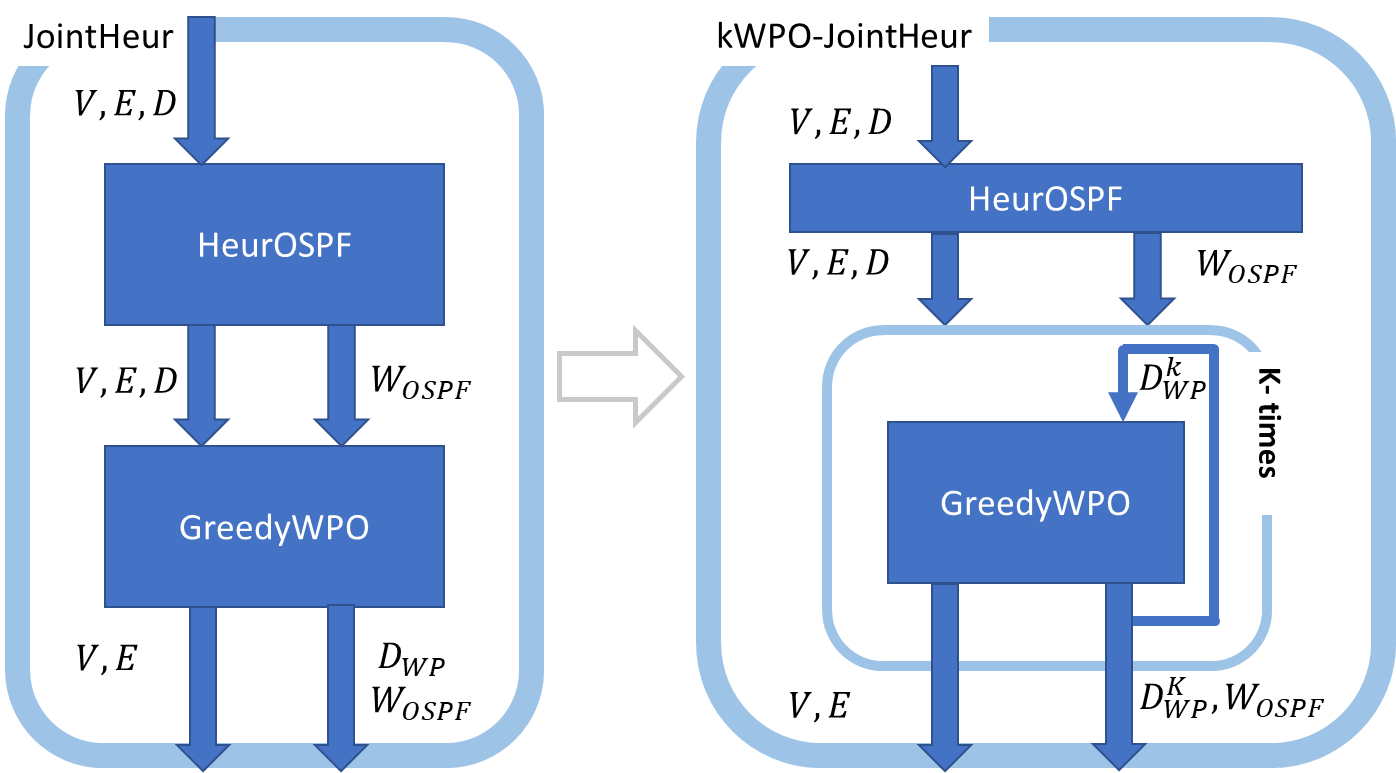
\includegraphics[width=\linewidth]{abbildungen/kWPO_Concept.png}
  \caption{Konzept von kWPO-JointHeur}
  \Description{A woman and a girl in white dresses sit in an open car.}
\end{figure}

\begin{figure}[h]
  \centering
  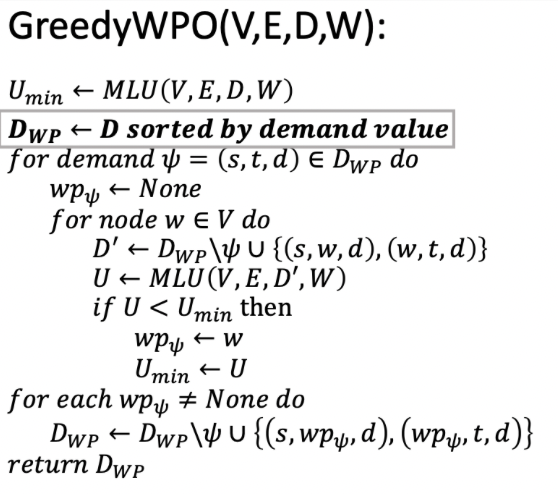
\includegraphics[width=\linewidth]{abbildungen/pseudo1}
  \caption{Pseudocode zu kWPo-JointHeur}
\end{figure}
Zur weiteren Optimierung von kWPO-JointHeur betrachten wir die GreedyWPO-Komponente genauer. In dieser Routine werden die Anfragen zunächst nach ihrem Volumen sortiert und dann in dieser Reihenfolge hinsichtlich der Wegpunkte bearbeitet. Es fällt auf, dass die Reihenfolge einen Einfluss auf die Performance haben muss, da bereits gesetzte Wegpunkte nicht gelöscht werden und unbearbeitete Anfragen nicht berücksichtigt werden. Jedoch berücksichtigt das verwendete Sortierkriterium nicht die zugrunde liegende Topologie.
Neben dem Anfragevolumen führen wir das zusätzliche Sortierkriterium der Knotenkapazität ein. Die Knotenkapazität eines Knoten sei durch die Summe der verbundenen Kantenkapazitäten gegeben.
Wie definieren die Knotenkapazität $C_v$ wie folgt: \begin{center} $c_v = \sum_{e_{v_{i}} \in E} c(e_{v_i})$\end{center}
Im Rahmen von kWPO-JointHeur, sollen die Anfragen nun nach der Summe der Quellen- und Senkenknotenkapazität absteigend sortiert werden. Die Begründung liegt in der Tatsache, dass Knotenpaare mit hoher Kapazität durch alternative Wege hoher Kapazität entsprechend die MLU stärker senken können[1].
\begin{figure}[h]
  \centering 
  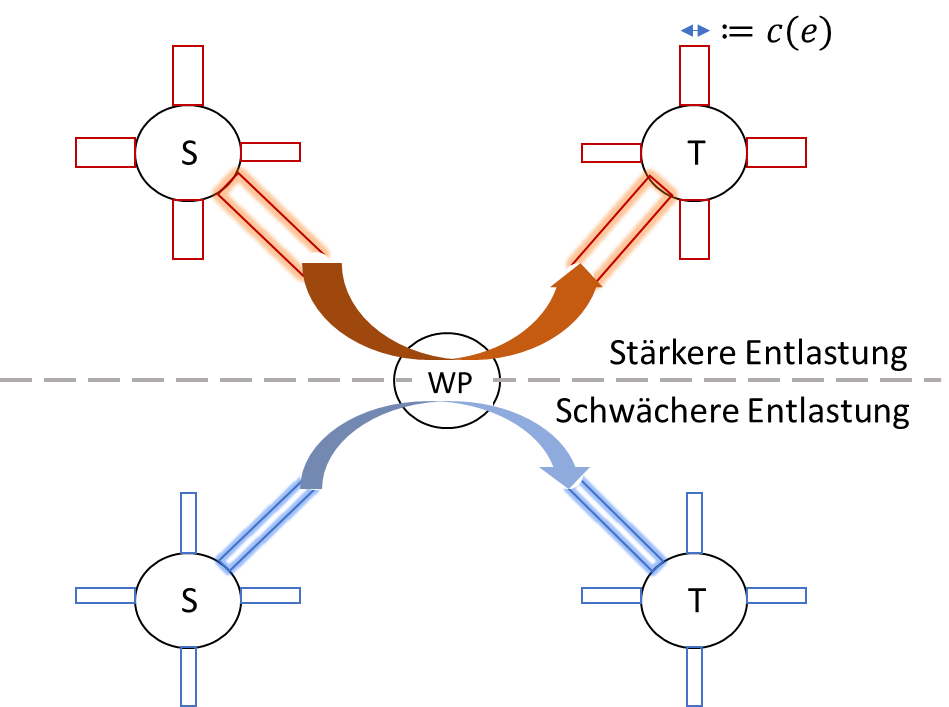
\includegraphics[width=\linewidth]{abbildungen/kWPO_Capacity.png}
  \caption{Einfluss der Knotenpakazität auf MLU}
 \end{figure}

\begin{figure}[h]
  \centering 
  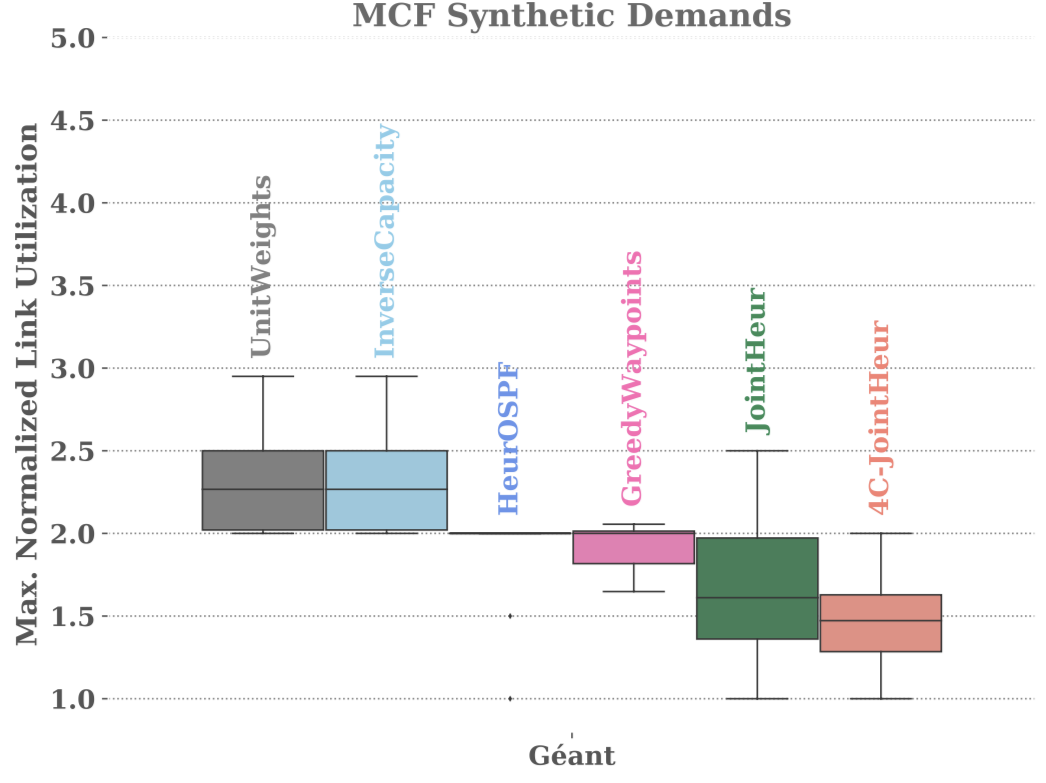
\includegraphics[width=\linewidth]{abbildungen/PNG-Bild}
  \caption{4C-JointHeur bei Verwendung synthetischer Demands}
 \end{figure}
Ein erstes Beispiel für die Effektivität dieser Abwandlung kann in Abbildung 3 betrachtet werden. So kann bei einer Sortierung nach Capacity und mit dem Parameter $k=4$ auf künstlichen Demands ein besseres Ergebnis erreicht werden als mit dem klassischen JointHeur. 
\begin{figure}[h]
  \centering 
  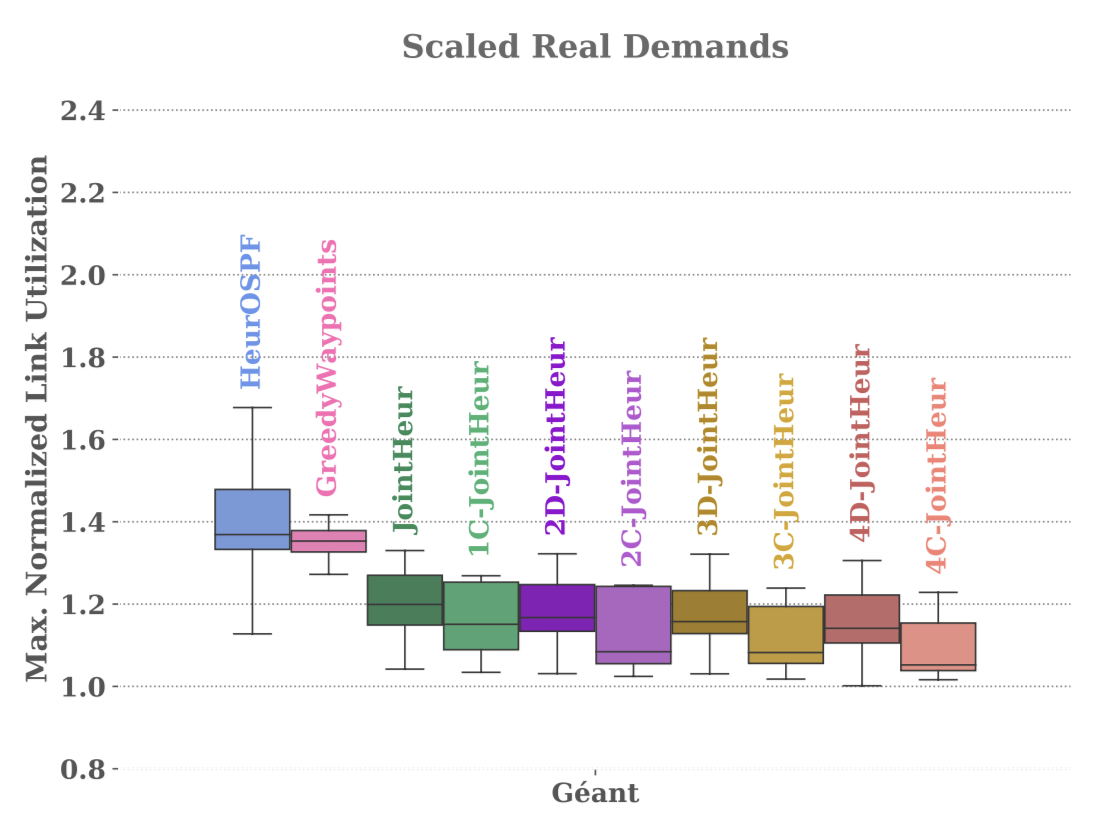
\includegraphics[width=\linewidth]{abbildungen/PNG-Bild 2}
  \caption{Verschiedene D- und C-JointHeur bei Verwendung tatsächlicher Demands}
  \Description{A woman and a girl in white dresses sit in an open car.}
\end{figure}
In Abbildung 4 werden die Abwandlungen mit den Parametern 1,2,3 und 4 betrachtet. Zusätzlich wird zu jedem dieser Fälle auch die Sortierung nach Capacity gegenübergestellt. Für das Ergebnis wurden echte Anfragen hinsichtlich ihres Volumens skaliert. Neben der Beobachtung, dass die Sortierung nach Capacity durchaus einen Unterschied macht, wird auch deutlich, dass mit höheren Werten für k auch eine bessere MLU einhergeht. In Abbildung 3 wird das Ergebnis für die Abwandlung 4C des JointHeur nochmal auf weiteren Topologien getestet und erreicht fast überall dort bessere Ergebnisse[1].
\begin{figure}[h]
  \centering 
  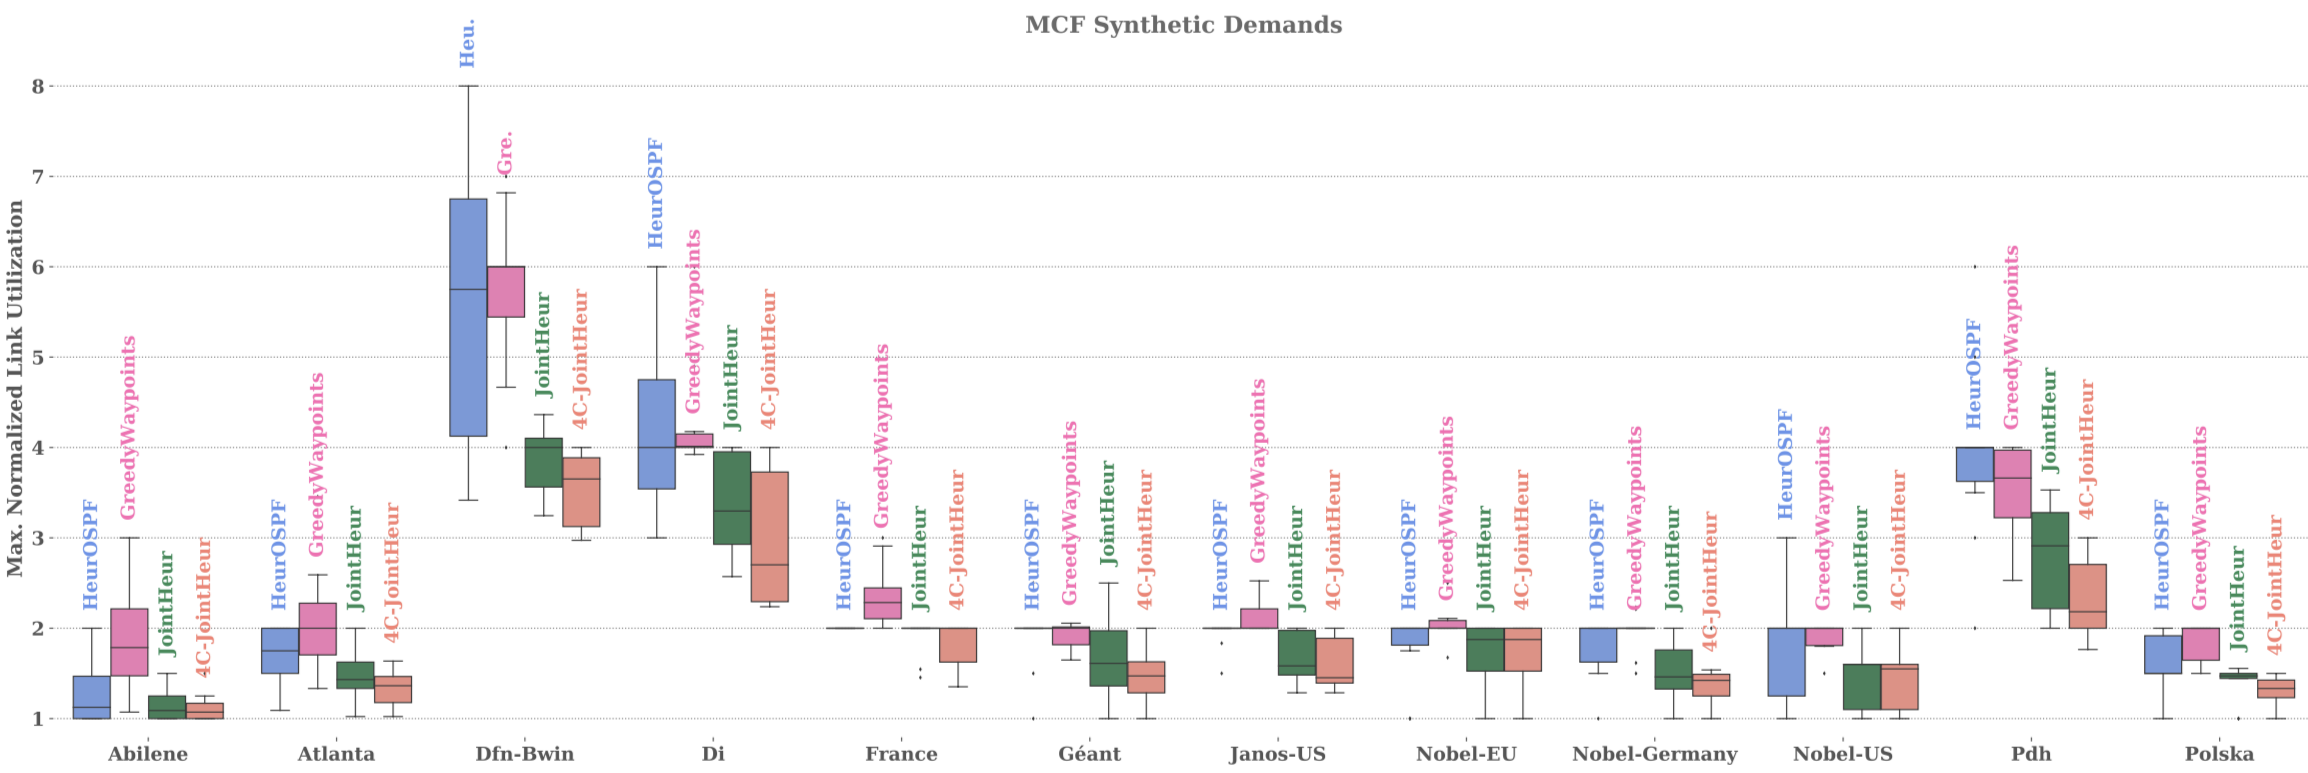
\includegraphics[width=\linewidth]{abbildungen/PNG-Bild 3}
  \caption{Vergleich von 1D- und 4C-JointHeur auf verschiedenen Topologien}
  \Description{A woman and a girl in white dresses sit in an open car.}
\end{figure}



\subsection{Topo-kWP-JointHeur}
Während wir mit der ersten Idee JointHeur um mehr Waypoints je Demand erweitert haben schränken wir mit Topo-kWP-JointHeur die nutzbaren Waypoints für die gesamte Topologie ein.
Durch diese Abwandlung kann der tatsächliche Einfluss der Waypoints auf die Performance von JointHeur besser veranschaulicht werden. Eine Steigerung der Performance, in diesem Fall also der MLU, kann durch diese Abwandlung offensichtlich nicht erwartet werden. 
Bestenfalls kann, bei entsprechend hohen Werten für die Beschränkung, das gleiche Ergebnis wie beim normalen JointHeur erreicht werden.
Daher steht bei dieser Abwandlung eher im Vordergrund, für welche Beschränkungswerte und damit einhergehend wie stark, sich die Performance beeinflussen lässt. \\
\\
Die praktische Abwandlung im Code ist simpel - Es muss lediglich ein Parameter $k$ in die 
GreedyWPO-Komponente des JointHeur-Algorithmus eingepflegt werden. $k$ fungiert dann als ein runter zählender Counter. Sollte GreedyWPO
einen Waypoint wählen, so würde k verringert, bis k am Ende 0 beträgt. Somit kann sichergestellt werden, dass nur die
erlaubte Anzahl an Wegpunkten erzeugt wird[1,2].
\\
\begin{figure}[h]
  \centering
  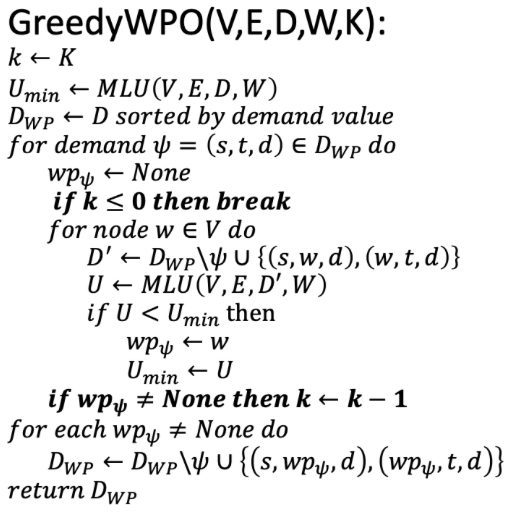
\includegraphics[width=\linewidth]{abbildungen/pseudo2}
  \caption{Pseudocode zu Topo-kWP-JointHeur}
\end{figure}
Nach der Implementierung haben wir den abgewandelten Algorithmus für mehrere Werte für $k$ ausgeführt. Die folgenden Plots stellen die interessantesten Werte dar:
\begin{figure}[h]
  \centering
  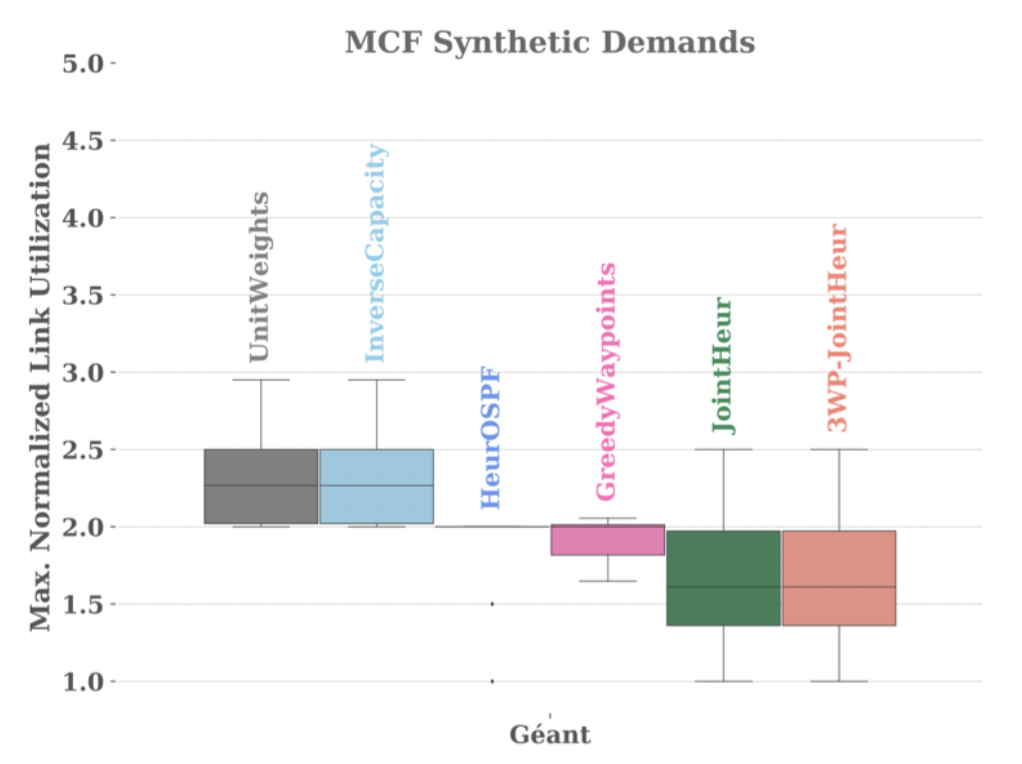
\includegraphics[width=\linewidth]{abbildungen/syntDemtopokwp}
  \caption{3WP-JointHeur auf der Topologie Geant mit künstlichen Demands}
\end{figure}
Die erste Abbildung dieses Unterkapitels zeigt die Resultate von Topo-kWP-JointHeur mit einer Beschränkung von $k = 3$. es würden künstliche Demands und die Topologie Geant verwendet.
Offensichtlich kann in diesem Fall mit $k = 3$ genau die Performance von JointHeur arbeiten. Für höhere Werte von $k$ wird genau das selbe Ergebnis erzielt, somit 
nutzt JointHeur in diesem Fall nicht mehr als 3 Wegpunkte auf dem Weg durch die Topologie. \\
Die darauf folgende Abbildung zeigt dagegen die Verwendung echter Demands mit mehreren möglichen Werten für $k$. Offensichtlich verbessert sich die MLU mit jedem weiteren nutzbaren Waypoint. 
Die Abbildung verdeutlicht den Einfluss der Waypoints auf die MLU-Performance von JointHeur sehr gut. 
\begin{figure}[h]
  \centering
  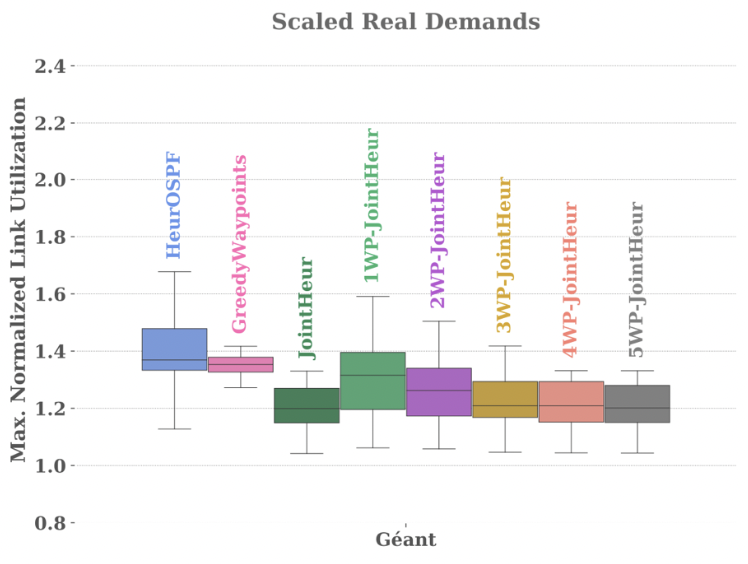
\includegraphics[width=\linewidth]{abbildungen/realDemtopokwp}
  \caption{3WP-JointHeur auf der Topologie Geant mit realen Demands}
\end{figure}
Um herauszufinden, mit welcher möglichst kleinen Waypoint-Beschränkung eine minimale MLU erreicht werden kann, haben wir die Beschränkungen auch 
auf mehreren Topologien betrachtet. Dies wird in der nächsten Abbildung dargestellt. Es hat sich dabei herausgestellt, dass mit einer Beschränkung von 3 Wegpunkten in den meisten Fällen
die Ergebnisse des unbeschränkten JointHeur erreicht werden können. Es folgt daraus, dass die meisten Topologien höchstens 3 Wegpunkte erzeugen und nutzen.
Es gab jedoch auch Topologien, auf welchem  3WP-JointHeur schlechter performt hat, darunter Janos-US, Nobel-Germany oder Polska. In diesem Fall
konnten offensichtlich wichtige Wegpunkte aufgrund der Beschränkung nicht erzeugt werden.
\begin{figure}[h]
  \centering
  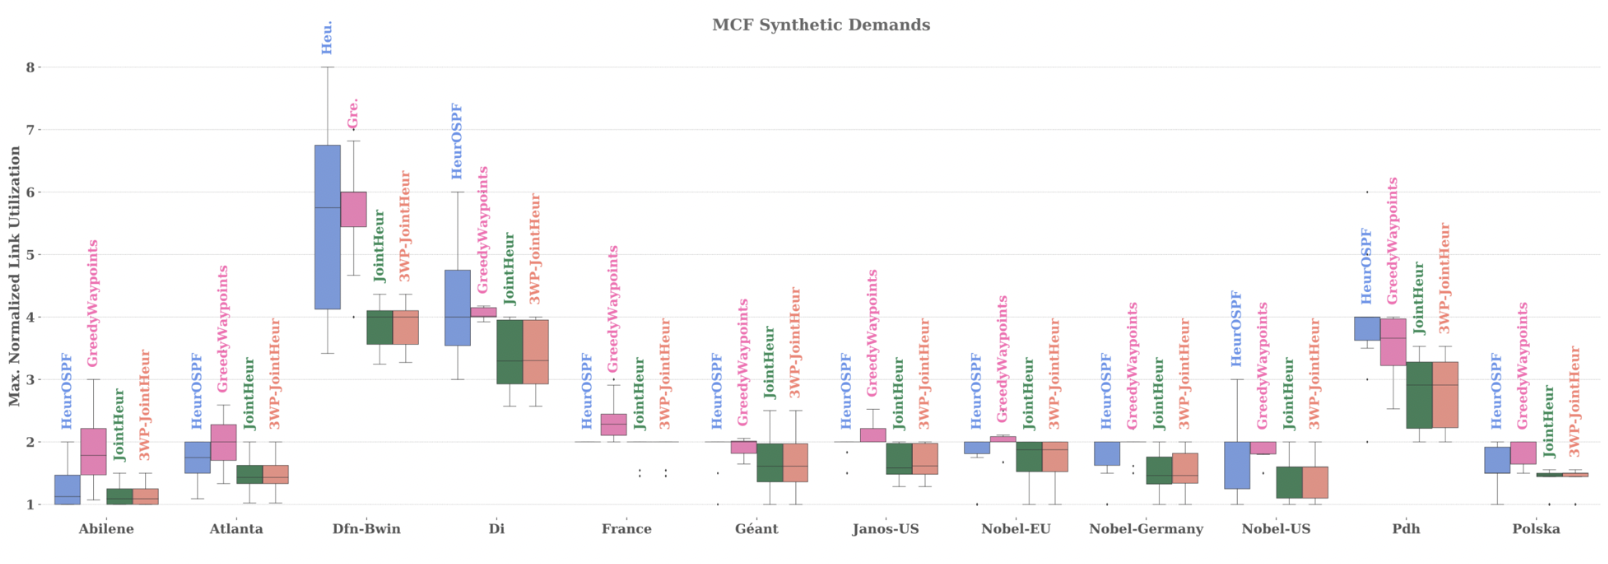
\includegraphics[width=\linewidth]{abbildungen/allTopologieskwp}
  \caption{3WP-JointHeur im Vergleich auf allen Topologien}
\end{figure}

\subsection{Nodes-kWP-JointHeur}
In unserer dritten Abwandlung betrachten wir ebenfalls eine Beschränkung der nutzbaren Wegpunkte, dieses Mal jedoch auf einzelne Knoten und nicht auf die gesamte Topologie bezogen.
Ein Array $K$ ordnet jedem Knoten $v$ einen Parameter $k_v$ (im Folgenden allgemein als $k$ bezeichnet) zu, welcher angibt, wie oft dieser Knoten als Wegpunkt verwendet werden darf. Hierbei ist insbesondere interessant, welchen Einfluss die verschiedenen Werte für $k$ auf die Performance haben und ob es sinnvoll und durchsetzbar ist, bestimmte Nodes durch $k=0$ zu sperren, sodass diese nicht als Wegpunkt fungieren können.
\\
\\
Ein Problem bei der Implementierung ist jedoch, geeignete Werte für $K$ zu finden. Welche Werte überhaupt gültig sind, hängt von der Topologie ab und kann somit grundsätzlich nicht verallgemeinert werden. Damit es trotzdem für alle Topologien einheitlich und leicht generierbar ist und weil uns insbesondere das Sperren von Knoten interessiert hat, haben wir uns in der praktischen Umsetzung dafür entschieden, jeden $c_{gen}$-ten (wobei $c_{gen} \in N$) Knoten beliebig oft als Wegpunkt zu erlauben und die anderen Knoten als Wegpunkte zu sperren ($k=0$). So sind z. B. bei  $c_{gen} = 4$ 75\% der Knoten gesperrt, während 25\% der Knoten beliebig oft als Wegpunkte verwendet werden dürfen. Im Folgenden sprechen wir auch von einer $\frac{1}{c}$-JointHeur[1,2].


\begin{figure}[h]
  \centering
  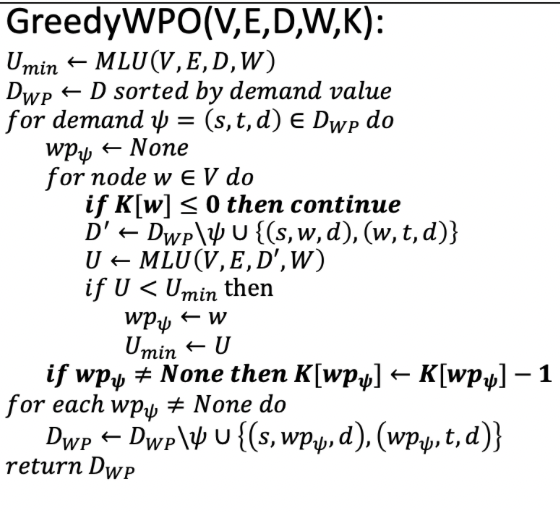
\includegraphics[width=\linewidth]{abbildungen/pseudo3}
  \caption{Pseudocode zu Nodes-kWP-JointHeur}
\end{figure}

\begin{figure}[h]
  \centering
  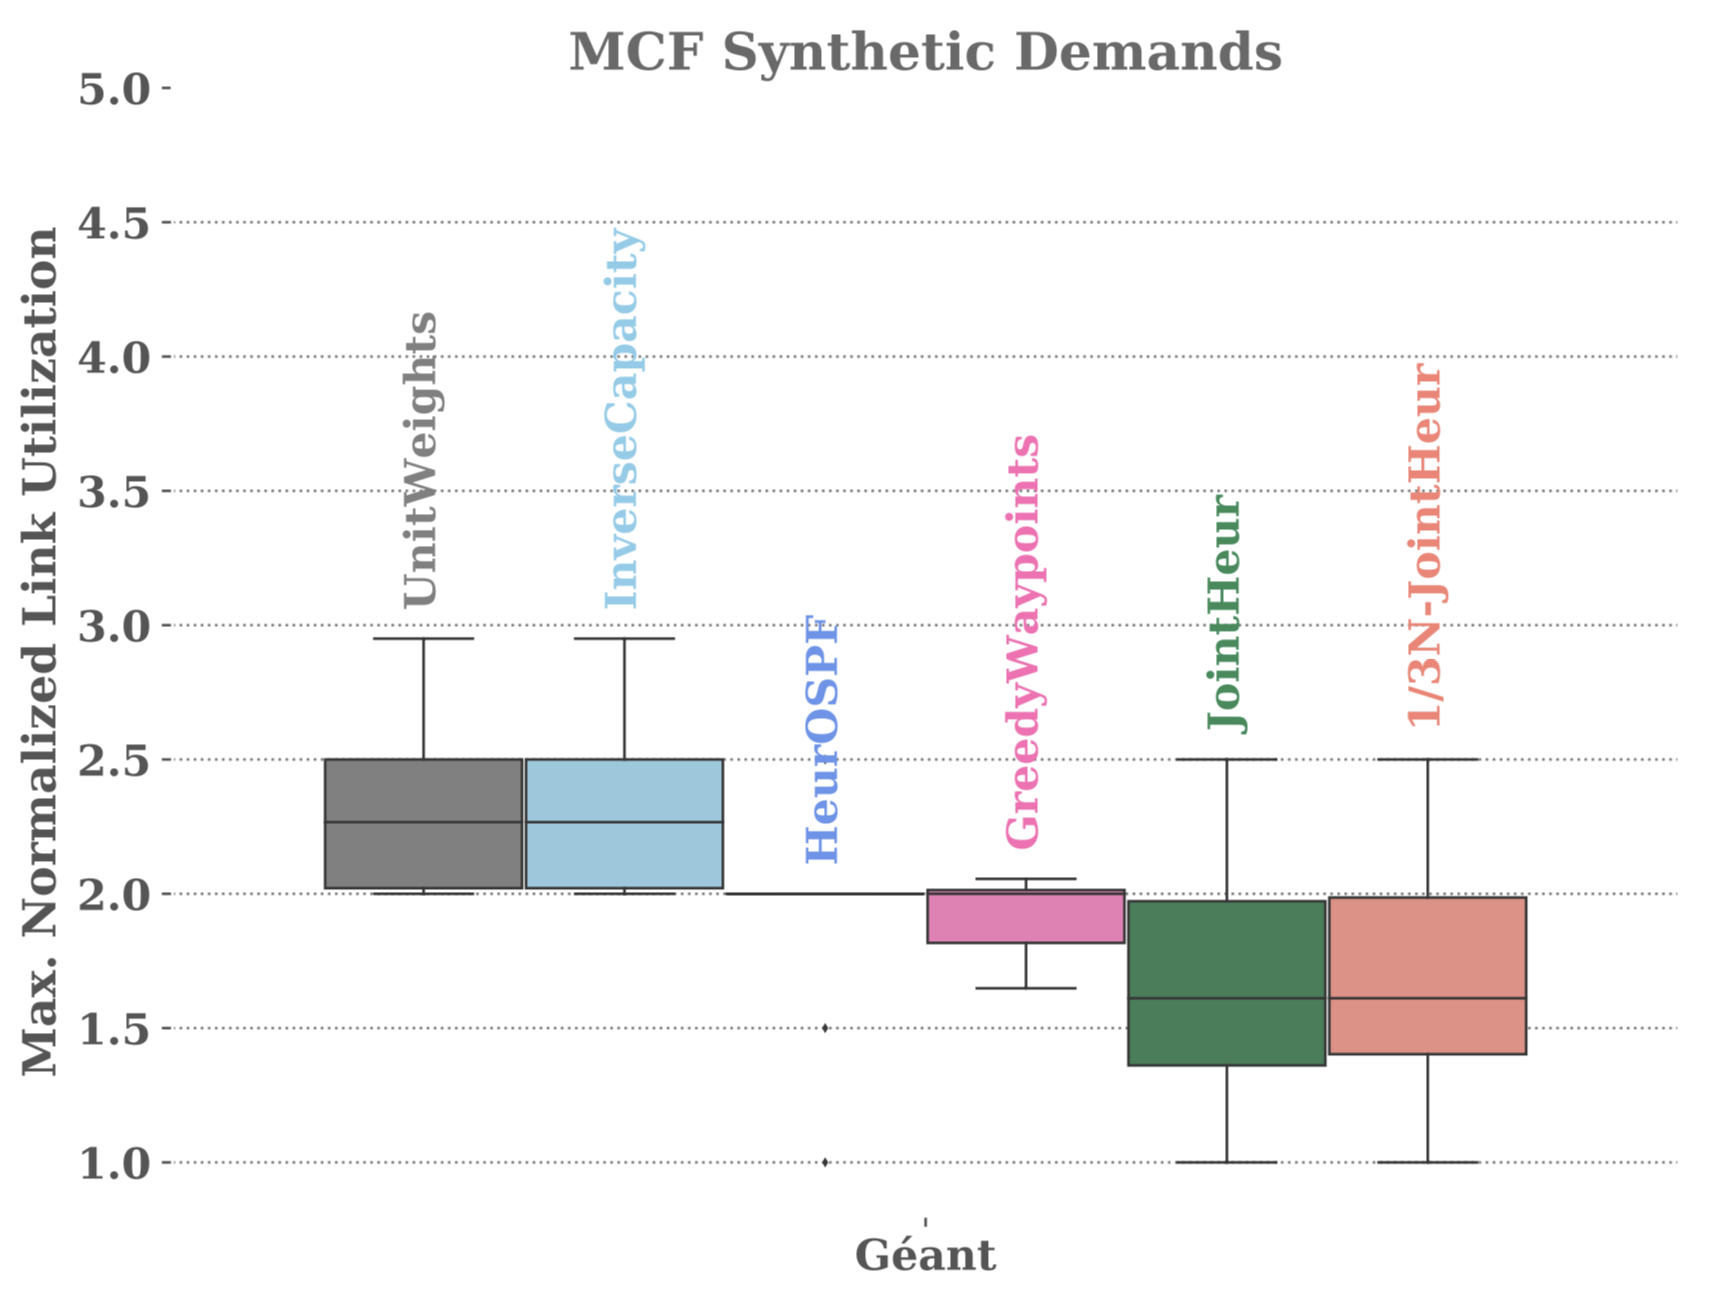
\includegraphics[width=\linewidth]{abbildungen/a31}
  \caption{1/3N-JointHeur auf künstlichen Demands im Vergleich}
\end{figure}


\begin{figure}[h]
  \centering
  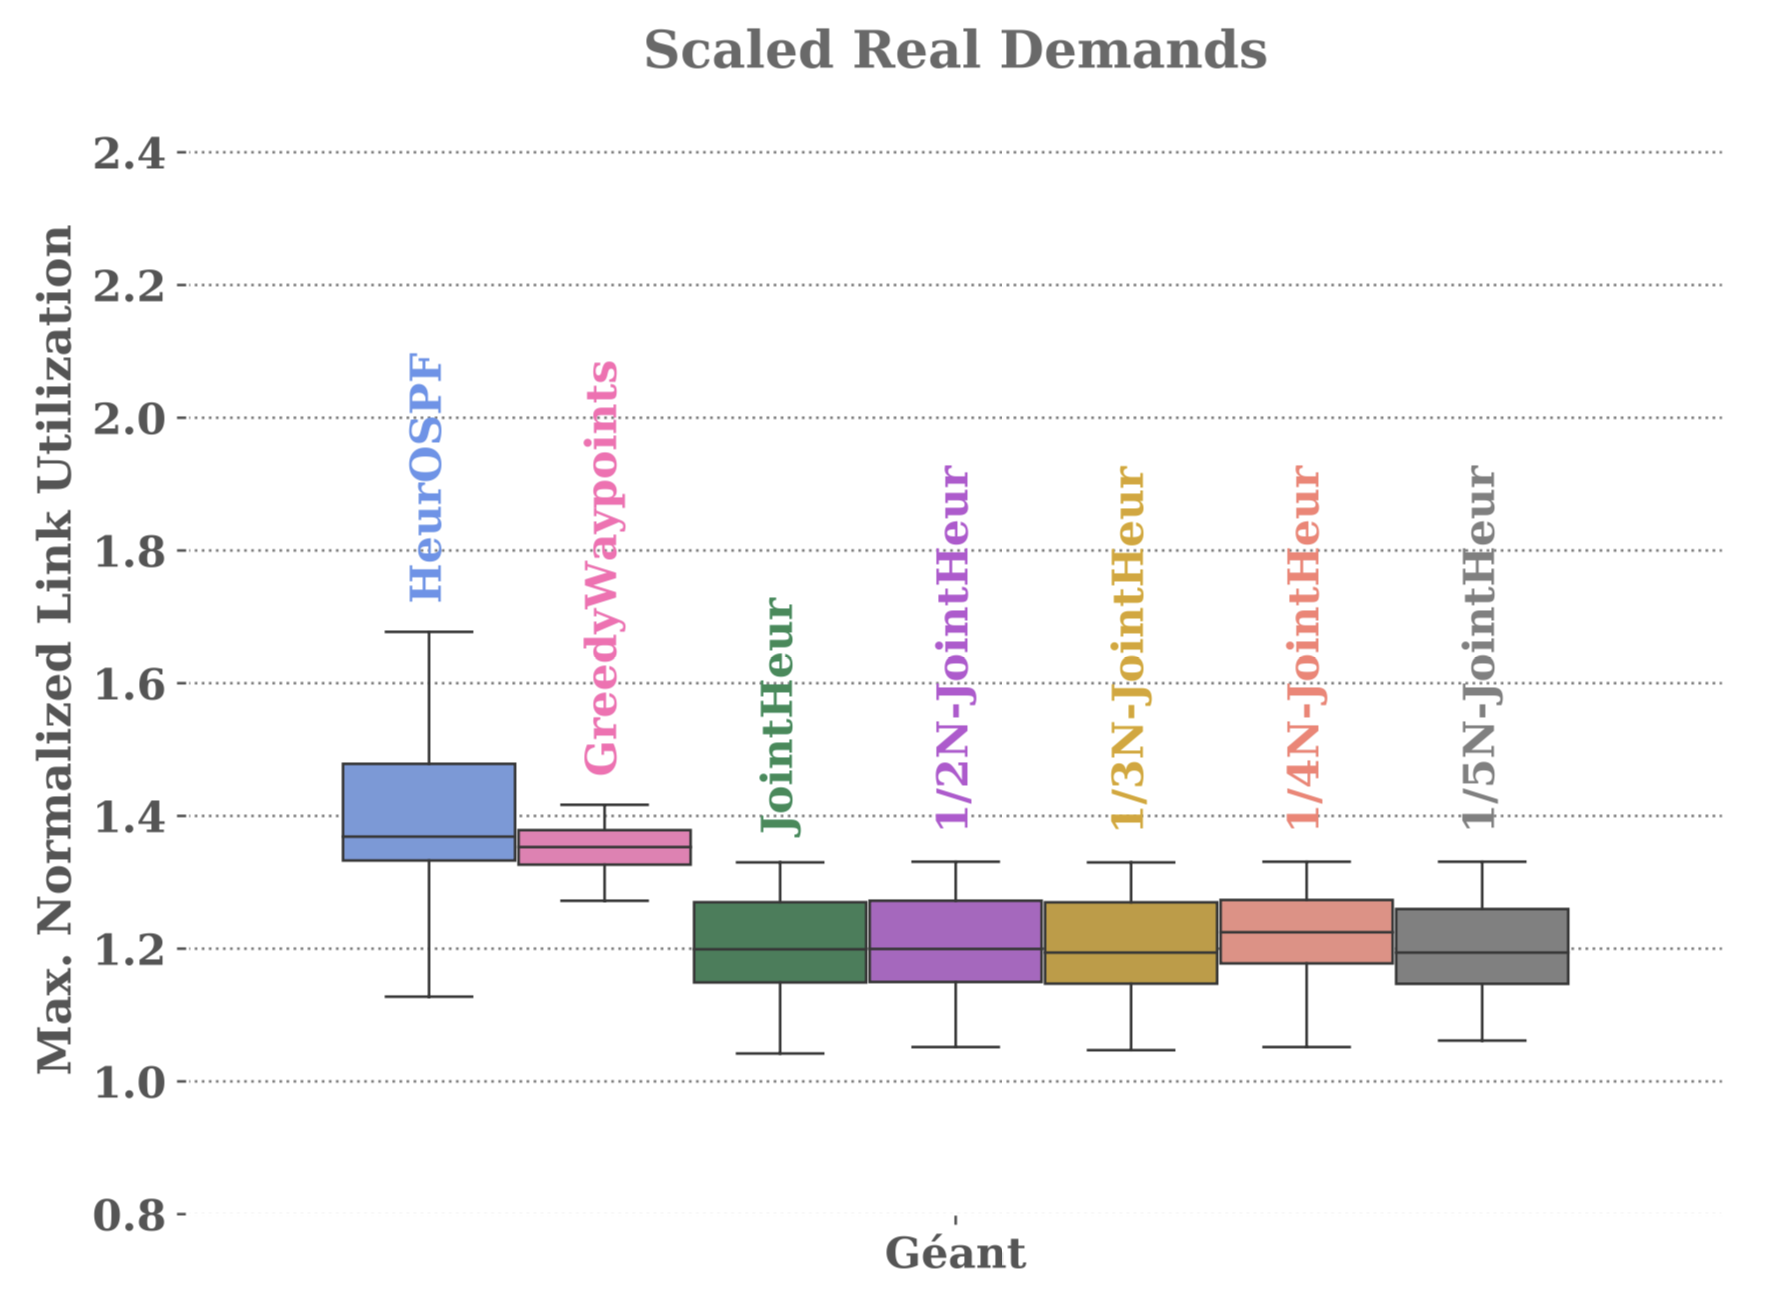
\includegraphics[width=\linewidth]{abbildungen/a32}
  \caption{1/k-JointHeur für verschiedene Werte und realen demands}
\end{figure}

Wie sich anhand der Durchführung auf der Topologie Geant erkennen lässt, wird, obwohl für ein größeres $c_{gen}$ der Pool an Wegpunkten kleiner wird, das Ergebnis nicht zwingend schlechter. Der Grund dafür ist, dass auch bei einem größeren  $c_{gen}$ Wegpunkte nicht gesperrt sein können, die bei einem kleineren  $c_{gen}$ gesperrt sind. So sieht man z. B. in Abbildung 10, dass  1/5N-JointHeur besser als 1/4N-JointHeur performt[1].

\begin{figure}[h]
  \centering
  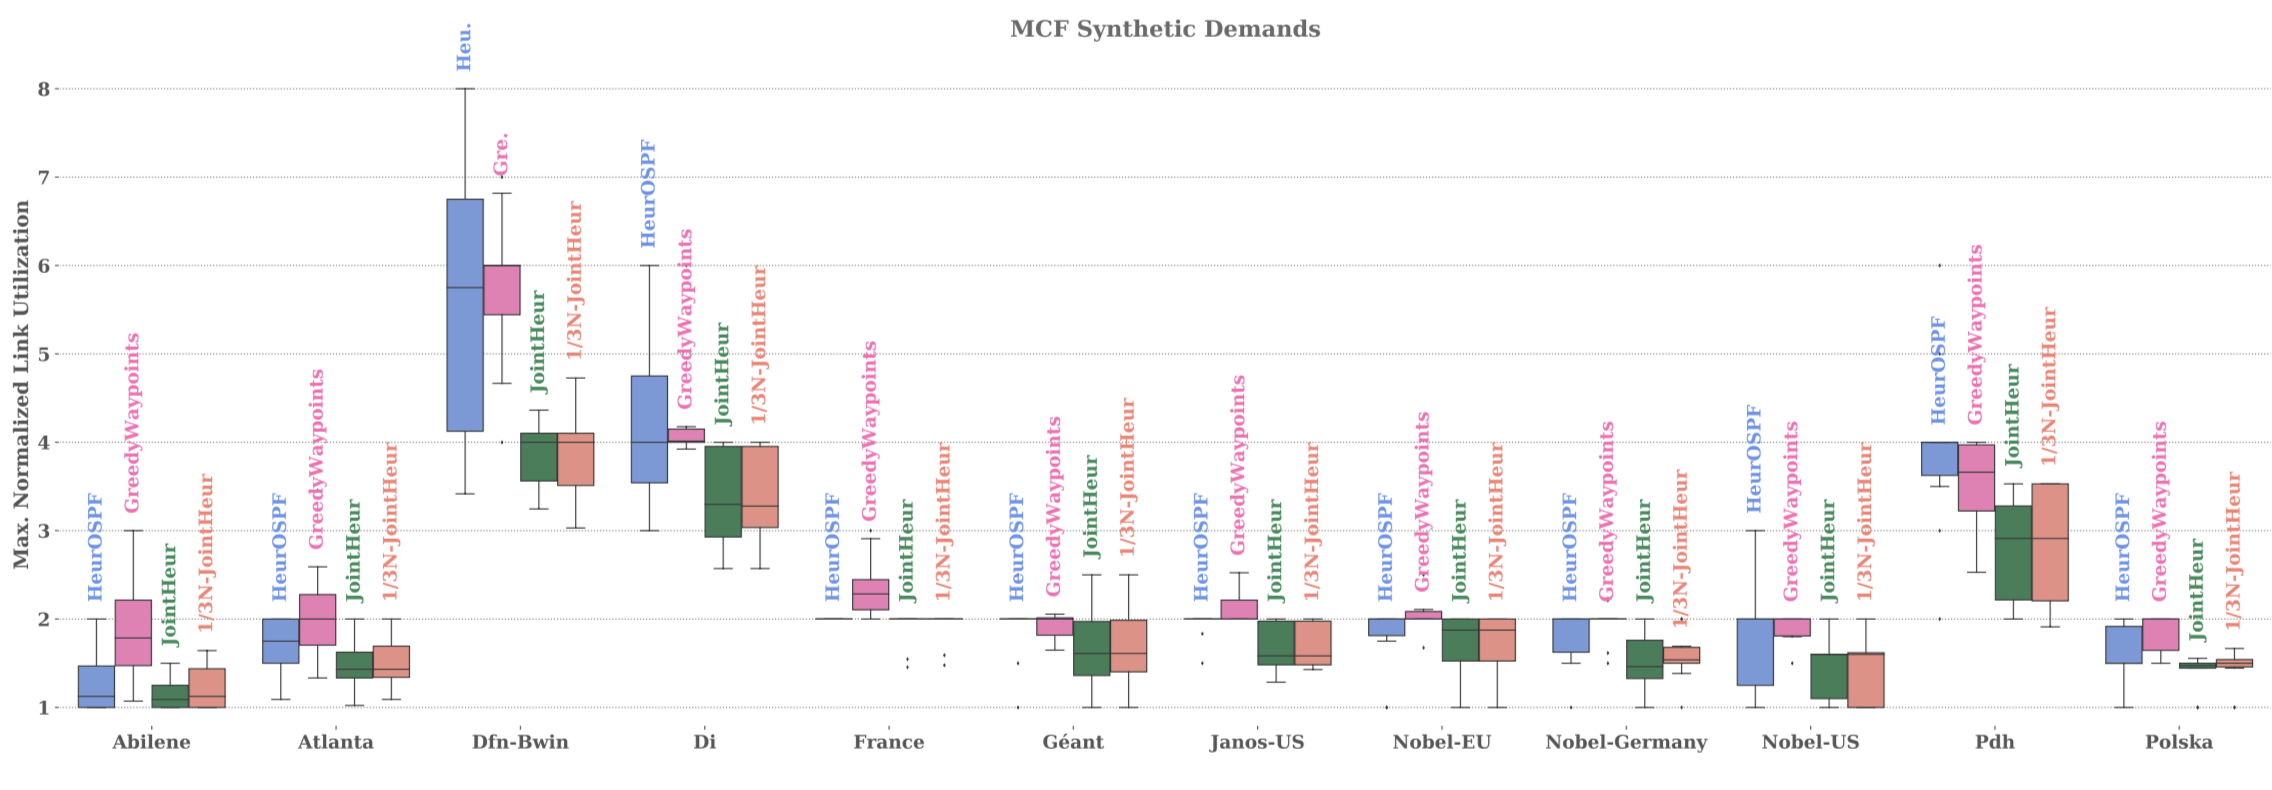
\includegraphics[width=\linewidth]{abbildungen/a33}
  \caption{1/3N-JointHeur auf verschiedenen Topologien getestet}
\end{figure}

In Abbildung 11 wird nochmal deutlich, dass die 1/3N-JointHeur nicht zwingend schlechter als JointHeur. Es hängt auch von der gewählten Topologie ab.


\section{Projekt 2 - Experimente in Mininet}
\subsection{Einführung}
Auch die zweite Reihe von Experimenten basiert auf dem genannten Paper. Allerdings stand hier nicht primär die Implementierung in Python im Vordergrund. Ziel der Experimente war es stattdessen,
unsere Abwandlungen aus Projekt 1 unter möglichst echten Bedingungen zu testen. Für die Simulation des Netzes haben wir keine tatsächliche Hardware verwendet.
Stattdessen haben wir ein in Nanonet implementiertes Simulationsframework genutzt, um im Linux-Kernel ein realistisches Netzwerk abzubilden und das Verhalten der Algorithmen unter realen Bedingungen zu testen. Ziel war es zudem, unsere Ideen durch geeignete Skalierungen möglichst gut dastehen zu lassen[1].

\subsection{Vorbereitung}
Um die beschriebenen Experimente durchzuführen, musste zunächst die Nanonet-Umgebung eingerichtet werden. Die Instruktionen aus dem zugehörigen GitHub-Repository konnten hierfür genutzt werden, jedoch stießen wir an mehreren Stellen auf Probleme. Unter kamen wir zum Schluss, dass die Linux-Umgebung bestimmte Vorrausetzungen erfüllen sollte. Insbesondere konnten wir die Experimente nicht in einer Linux-Umgebung starten, die auf dem Windows-Subsystem basiert.

\subsection{kWPO-JointHeur}
Der Algorithmus kWPO-JointHeur versucht einer Anfrage mehrere Wegpunkte zuzuweisen, um damit die Auslastung zu verbessern. Daher suchen wir eine Topologie, die von mehreren Wegpunkten profitieren kann. Dazu modifizieren wir die Joint-Topologie, die bereits im ursprünglichen Paper verwendet wurde. Durch die Duplizierung eines Teilbereiches dieser Topologie, entsteht eine zweiter Bereich, welcher für Wegpunkte empfänglich wird[1].
\begin{figure}[h]
  \centering
  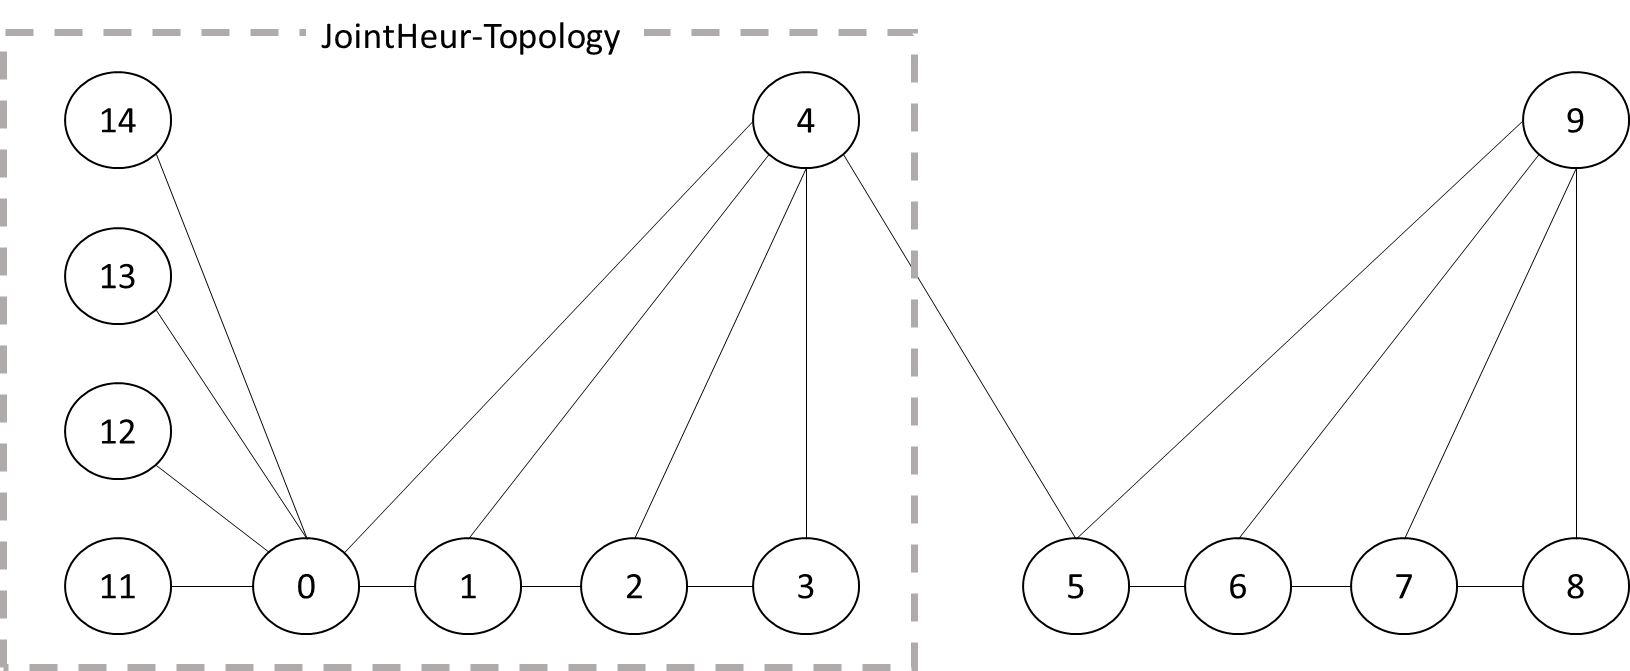
\includegraphics[width=\linewidth]{abbildungen/kWPO_topo.png}
  \caption{Topologie für kWPO-JointHeur-Experiment}
\end{figure}

\begin{figure}[h]
  \centering
  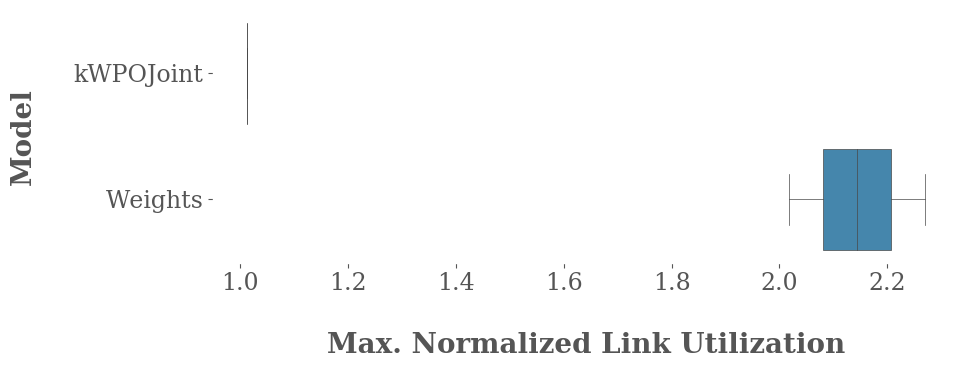
\includegraphics[width=\linewidth]{abbildungen/kWPOJoint_Plot.png}
  \caption{Ergebnis des Experiments}
\end{figure}
In Abbildung 13 können wir sehen, dass die Konfiguration mit 2 Wegpunkten einen sehr viel besseren MLU-Wert erzeugt, als die Steuerung über die reine Gewichtung von Kanten.

\subsection{Topo-kWP-JointHeur}
Unsere zweite Abwandlung konnte recht einfach implementiert werden. Zur Erinnerung: bei der zweiten Idee geht es um die Beschränkung der nutzbaren Waypoints für die gesamte Topologie. Da diese Abwandlung niemals zu einer besseren MLU führen kann, wird das Resultat dieses Algorithmus nicht besonders gut dargestellt, sondern eher schlecht.
Für die Implementierung dieser Idee haben wir die Joint-Topologie verwendet, welche im zugehörigen Repository des Base-Paper gegeben war. In dieser haben wir dann einen Waypoint unbrauchbar gemacht, um eine Beschränkung zu simulieren. Das Resultat kann auf folgender Abbildung betrachtet werden:

\begin{figure}[h]
  \centering
  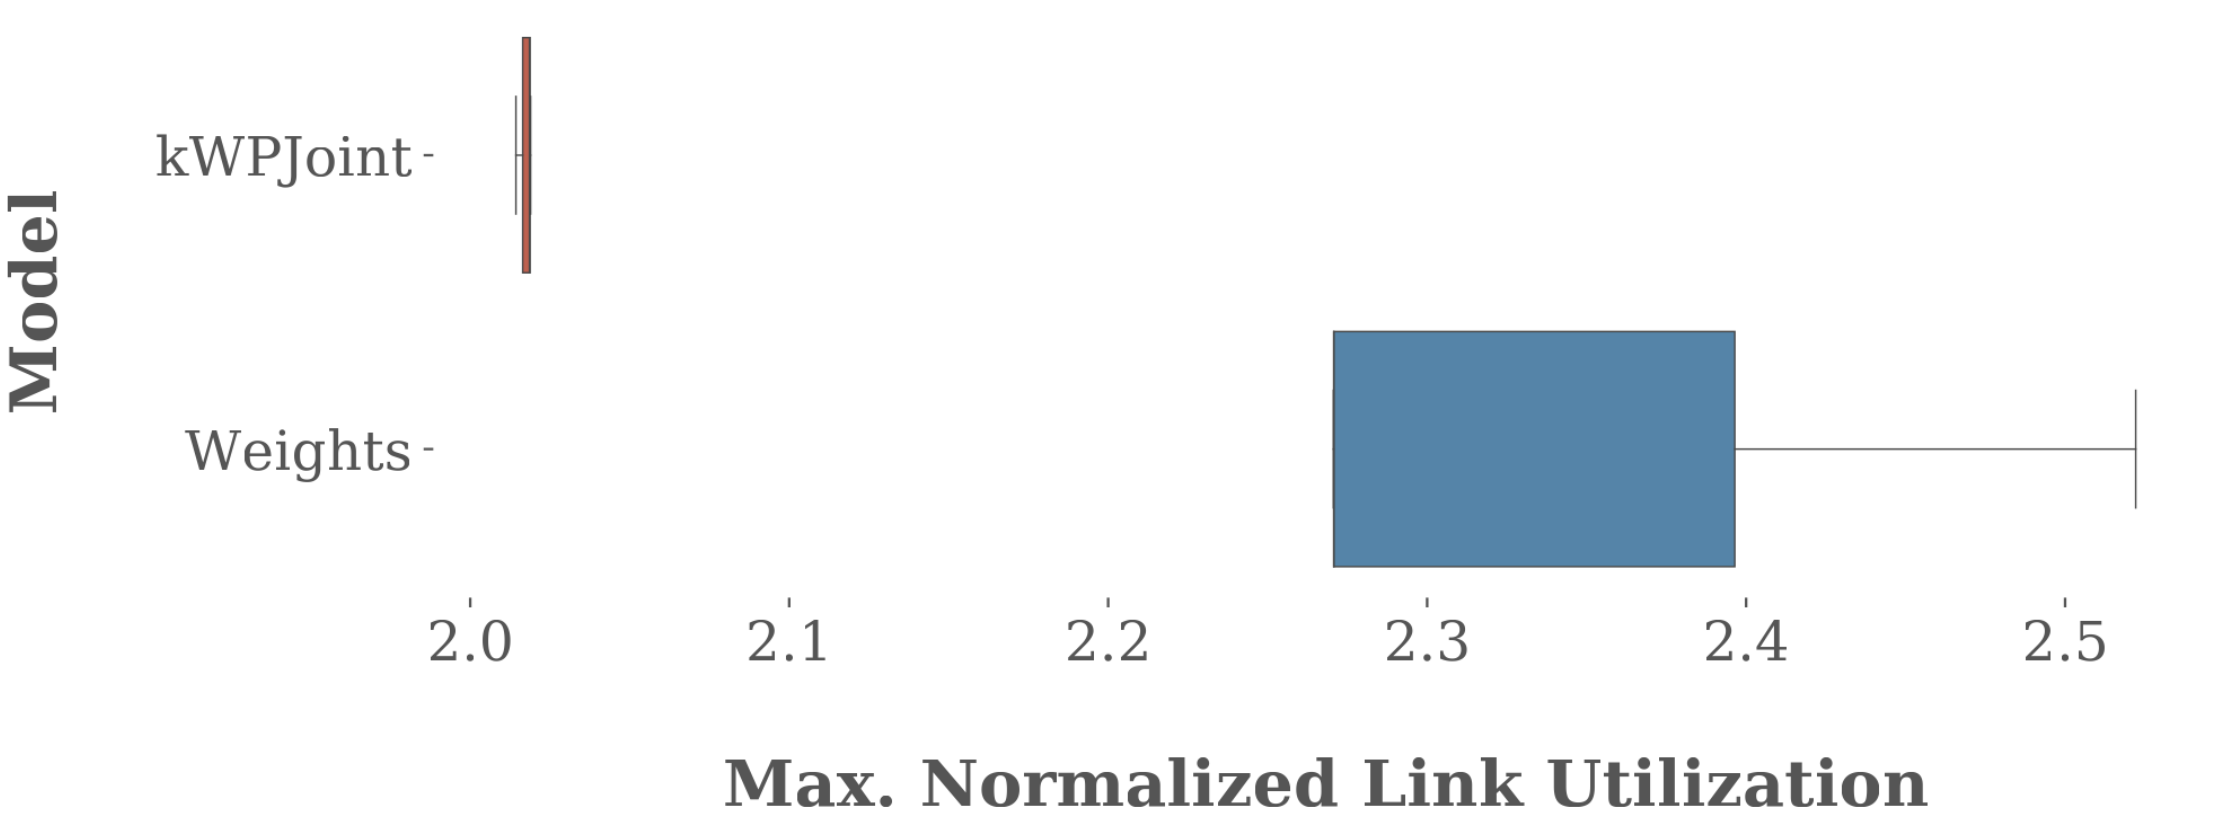
\includegraphics[width=\linewidth]{abbildungen/22}
  \caption{Resultat von kWP-JointHeur}
\end{figure}
Wie in den Abbildungen 9 und 10 erkennbar
Offensichtlich führt die schon das entfernen eines Waypoints zu einer deutlichen Rechtsverschiebung im Plot und somit zu einer Verschlechterung der MLU auf über 2.0.

\subsection{Nodes-kWP-JointHeur}
Der dritte Algorithmus, Nodes-kWP-JointHeur, basiert auch auf der Einschränkung der Wahl der Wegpunkte. Dabei liegt der Fokus nicht auf der Anzahl, sondern der Beschaffenheit der Wegpunkte. Im Rahmen der praktischen Umsetzung für unsere Mininet-Experimente werden wir hier in Anlehnung zum zweiten Algorithmus eine bestimmte Zahl an beliebigen Wegpunkten aus der bereits gegebenen Netzwerk-Instanz für die JointHeur entfernen. Im Gegensatz zum zweiten Algorithmus entfernen wir nun jedoch mehrere Wegpunkte, sodass eine noch schlechtere Auslastung zu erwarten ist.

\begin{figure}[h]
  \centering
  \includegraphics[width=\linewidth]{abbildungen/kWPnJoint.png}
  \caption{Resultat von kWPn-JointHeur}
\end{figure}

In Abbildung 18 sind die Ergebnisse der Mininet-Evaluation für dieses Szenario abgebildet. Es fällt auf, dass der dritte Algorithmus eine schlechtere Auslastung vorweist, als die reine Steuerung über die Gewichtung. Dies ist jedoch nicht plausibel, da der Joint-Algorithmus eine Kombination aus idealer Gewichtung und zusätzlichen Wegpunkten darstellt. Durch die Entfernung von Wegpunkten sollte der Algorithmus aber weiterhin besser als die reine Gewichtung sein.

Die fehlerhaften Ergebnisse dürften auf die eingeschränkten Kapazitäten unseres Testrechners zurückzuführen sein.

\section{Replikation der Ergebnisse einer anderen Gruppe}
Zu Ende der Bearbeitungszeit fand jeweils ein sogenannter Code-Freeze statt, bei dem die teilnehmenden Gruppen ihre Arbeit untereinander bewerten und replizieren sollten. 
\subsection{Code-Freeze - Projekt 1}
Die Gruppe bot dabei zwei Wege an, ihre Experimente zu replizieren. Neben der Bereitstellungsform, in welchem auch der Code des Base-Papers bereitgestellt wird, ist auch eine vorkonfigurierte virtuelle Maschine verfügbar.
Die gegebenen Dateien konnten ohne Probleme ausgeführt werden. Typischerweise muss allerdings für die Ausführung auf durchschnittlicher Hardware viel Zeit eingeplant werden.
So dauerte die Ausführung des Experiments, welches mehrere Topologien nutzt, mehr als einen Tag. 
Die aus den Datei gewonnen Plots entsprachen denen, welche die Gruppe selbst angegeben hatte.
Zusätzlich zu den bestehenden Plotter wurde auch zusätzlich ein weiteres Diagramm erzeugt, 
welches die tatsächliche Ausführungszeit der Algorithmen darstellt. Allerdings hätte die Darstellung für die Ausführung bei künstlichen Demands besser skaliert sein können, da einige in der Legende genannten Algorithmen im Plot nicht zu sehen sind, siehe beispielsweise IndependentPathWaypoints [5]. 
\begin{figure}[h]
  \centering
  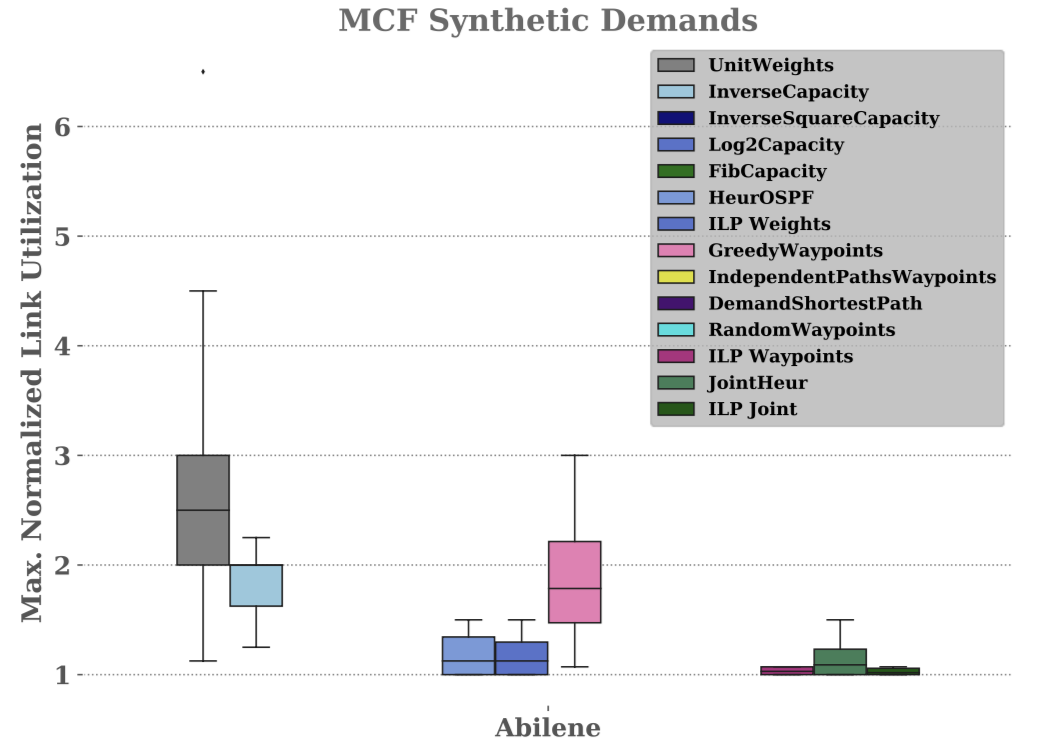
\includegraphics[width=\linewidth]{abbildungen/replik1}
  \caption{Beispielplot aus der Replikation der anderen Gruppe}
\end{figure}

\subsection{Code-Freeze - Projekt 2}
Auch das zweite Projekt der anderen Gruppe basierte auf den Grundideen von Projekt 1 und wurde in Form von Experimenten mit Nanonet durchgeführt. Auch hier ist wieder positiv anzumerken, dass der Code wieder zusätzlich zum bestehenden Weg auch über ein vorbereitetes VM-Image direkt ausgeführt werden kann. Die zur Ausführung nötigen Schritte sind zudem nochmal beschrieben. \\
Bei der reinen Ausführung des Codes hatten wir keine Probleme. Allerdings waren nachträglich einige Modifikationen an der Datei nötig, welche zum Plotten der Ergebnisse benötigt wird [6]. Nach den Modifikationen haben wir folgenden Boxplot erhalten:
\begin{figure}[h]
  \centering
  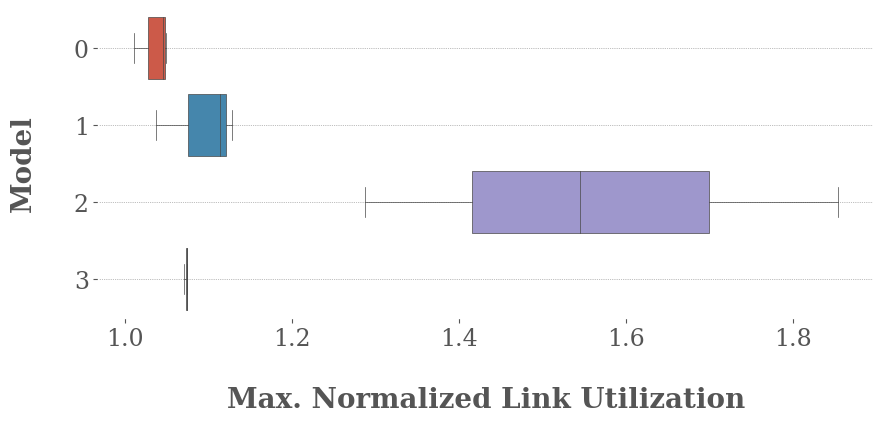
\includegraphics[width=\linewidth]{abbildungen/boxplot}
  \caption{Erzeugter Boxplot aus der zweiten Replikation}
\end{figure}

\section{Zusammenfassung und Ausblick}
Im Rahmen von Projekt 1 haben wir uns mit der Wahl von Wegpunkten beim Routing in Netzwerkinstanzen beschäftigt. Anhand unserer Ergebnisse kann geschlossen werden, dass der Einfluss von Wegpunkten sehr von der Beschaffenheit der Topologie und der Verteilungen der Anfragen abhängt. So konnte unsere Algorithmen in manchen Konstellationen unsere Zielmaße stark verbessern oder verschlechtern, aber in anderen Konstellationen trotz der investierten Rechenzeit keine Reaktion stimulieren.

Im zweiten Projekt konnten wir unsere Algorithmen in einer alternativen Umgebung testen. Hier konnten wir im Einklang mit unseren Erwartungen beim ersten Algorithmus eine optmierte und beim zweiten Algorithmus eine verschlechterte MLU feststellen. Die Ergebinisse zum dritten Algorithmus können wir jedoch aufgrund von mangelnder Plausibilität nicht berücksichtigen.

Für die Zukunft wäre eine Betrachtung der Kombination unserer Ideen interessant. Die Schwächen einer Idee können durch die jeweils anderen Ideen kompensiert werden. Eine Kombination der Algorithmen mit ihren Vorteilen und Nachteilen könnte wie folgt aussehen:\\
Die erste Idee bringt den Vorteil, dass die Anzahl der verwendeten Wegpunkte nach oben hin offen wird. Hier muss jedoch berücksichtigt werden, dass die Anzahl,k, der internen Iterationen keine Aussage über die Zahl der tatsächlich generierten Wegpunkte gibt.  Es ist also schwer vorhersehbar, wie viele Iterationen die Greedy-WPO Komponente idealerweise laufen sollte, um eine passende Zahl an Wegpunkten zu erhalten. \\
Hier kann die zweite Idee herangezogen werden. Eine möglichst hohe Zahl an internen Iterationen bei Idee 1 kann mit einer eingeschränkten Zahl an Wegpunkten in Anlehnnung an Idee 2 terminiert werden.\\
Im Rahmen dieser Kombination stellt sich die Frage: Die Zahl der Iterationen von GreedyWPO wird zwar flexibler, aber die zusätzliche Einschränkung kann möglicherweise wichtige Wegpunkte abschneiden und die die Zielfunktion negativ beeinflussen. Für eine Beschränkung $k$ der nutzbaren Waypoints war $MLU_{k}$ immer $\geq$ MLU. \\

Schließlich kann die dritte Idee herangezogen werden, um der Generierung von Wegpunkten eine Priorisierung einzuprägen. Dadurch können potenziell gute Wegpunkte in der Generierung vorgezogen werden. Es muss jedoch berücksichtigt werden, dass die Kriterien für die Bestimmung der Priorisierung, definiert durch $K$, nicht eindeutig sind und situationsbedingt festgelegt werden müssen.

\section{References}
1. M.Parham, T.Fenz, N.Süss, K-T Förster, S.Schmid. 2021 \\
Traffic Engineering with Joint Link Weight and Segment \\
Optimization \\
\\
2. T.Fenz \\
Simulationsframework zur praktischen Implementierung der Algorithmen aus dem Paper in Python \\
\url{https://github.com/tfenz/TE_SR_WAN_simulation} \\
\\
3. N.Süss \\
Simulationsframework zur Durchführung der Experimente in Nanonet \\
\url{https://github.com/nikolaussuess/TE_SR_experiments_2021} \\
\\
4. N.Süss \\
Zugehörige Nanonet-Version für die Experimente \\
\url{https://github.com/nikolaussuess/nanonet} \\
\\
5. S.Peters, M.Weiler, G.Karamoussanlis \\
Repository Projekt 1 \\
\url{https://github.com/JorgoJorgo/Fachprojekt} \\
\\
6. S.Peters, M.Weiler, G.Karamoussanlis \\
Repository Projekt 2 \\
\url{https://github.com/togir2/TE_SR_experiments_2021} \\
\\
Der gesamte zum Paper [1] zugehörige Code, der die Grundlage unserer Implementierungen ist, kann neben den oben genannten Links zusätzlich nochmal über \url{https://whatif-tools.net/segment-routing/} aufgerufen werden. \\







%%
%% The acknowledgments section is defined using the "acks" environment
%% (and NOT an unnumbered section). This ensures the proper
%% identification of the section in the article metadata, and the
%% consistent spelling of the heading.


%%
%% The next two lines define the bibliography style to be used, and
%% the bibliography file.

\appendix

%%
%% If your work has an appendix, this is the place to put it.
%%\appendix
\end{document}
%%\endinput
%%
%% End of file `sample-sigconf.tex'.
